\usetikzlibrary{arrows.meta,calc,patterns}

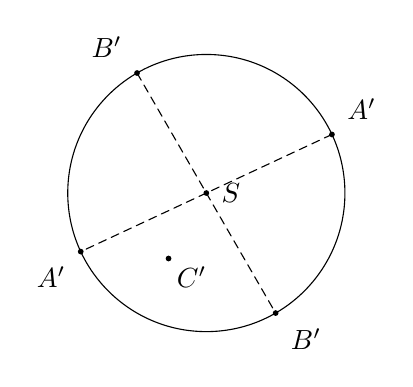
\begin{tikzpicture}[>=Stealth, line cap=round, line join=round, scale=0.8]

% ----------------------------
% PARAMETERS
% ----------------------------
\def\R{2.2}       % circle radius
\def\phiA{25}     % angle for A' pair
\def\phiB{120}    % angle for B' pair
\def\phiC{240}    % angle for C' (projection of C)

% ----------------------------
% HATCHED DISK
% ----------------------------
\draw (0,0) circle (\R);

% ----------------------------
% POINTS
% ----------------------------

% A' pair
\coordinate (A1) at ({\R*cos(\phiA)}, {\R*sin(\phiA)});
\coordinate (A2) at ({-\R*cos(\phiA)}, {-\R*sin(\phiA)});

% B' pair
\coordinate (B1) at ({\R*cos(\phiB)}, {\R*sin(\phiB)});
\coordinate (B2) at ({-\R*cos(\phiB)}, {-\R*sin(\phiB)});

% C' (inside the disk, not on boundary)
\pgfmathsetmacro{\rC}{1.2}  % distance from center
\coordinate (C1) at ({\rC*cos(\phiC)}, {\rC*sin(\phiC)});

% ----------------------------
% DASHED DIAMETERS
% ----------------------------
\draw[densely dashed] (A1) -- (A2);
\draw[densely dashed] (B1) -- (B2);

% ----------------------------
% CENTER POINT S
% ----------------------------
\fill (0,0) circle (1.3pt);
\node[right=2pt] at (0,0) {$S$};

% ----------------------------
% LABELS
% ----------------------------
\fill (A1) circle (1.3pt);
\node[above right=2pt] at (A1) {$A'$};
\fill (A2) circle (1.3pt);
\node[below left=2pt] at (A2) {$A'$};

\fill (B1) circle (1.3pt);
\node[above left=2pt] at (B1) {$B'$};
\fill (B2) circle (1.3pt);
\node[below right=2pt] at (B2) {$B'$};

\fill (C1) circle (1.3pt);
\node[below right=-0.5pt] at (C1) {$C'$};

\end{tikzpicture}
